\begin{frame}{Quantum GANs - Overview}
    \begin{center}
        \begin{tikzpicture}
            \node (figure) {\includegraphics[width=\linewidth,clip,trim=2.25cm 17.45cm 2.3cm 2.22cm,page=2]{figures/original-paper.pdf}};
            \node[xshift=-90, yshift=70] at (figure) {\tiny N 1 log M};
            % \node[xshift=-70, yshift=60] at (figure) {\tiny Batch GAN};
        \end{tikzpicture}
        % \hspace{-\linewidth}\frame{
        %     \begin{tikzpicture}
        %         \fill[blue] (0,0) rectangle (1cm,1cm);
        %     \end{tikzpicture}
        % }
        % \begin{tikzpicture}
            % \node (figure) {\includegraphics[width=\linewidth,clip,trim=2.25cm 17.45cm 2.3cm 2cm,page=2]{figures/original-paper.pdf}};
            % \draw (figure.north west) rectangle (3cm, 2cm);
        % \end{tikzpicture}
    \end{center}
\end{frame}

\begin{frame}{Quantum GANs - Details}
    \begin{center}
        \begin{tikzpicture}
            \node (figure) {\includegraphics[height=0.9\textheight,clip,trim=1.5cm 14cm 8.5cm 1.7cm,page=10]{figures/original-paper.pdf}};
            \node[xshift=-70, yshift=102] at (figure) {\tiny Patch GAN};
            \node[xshift=-70, yshift=-5] at (figure) {\tiny Batch GAN};
        \end{tikzpicture}
    \end{center}
\end{frame}